\subsection{IFIT1 Localisation in the Context of RSV pIBs and IBs} \label{subsec:IFIT1 Localisation in the Context of RSV pIBs and IBs}
\subsubsection{Nascent IFIT1 in a Simplified System of pseudo-IBs} \label{Nascent IFIT1 in a Simplified System of pseudo-IBs}
%293t hnhp

\begin{figure}
    \centering
    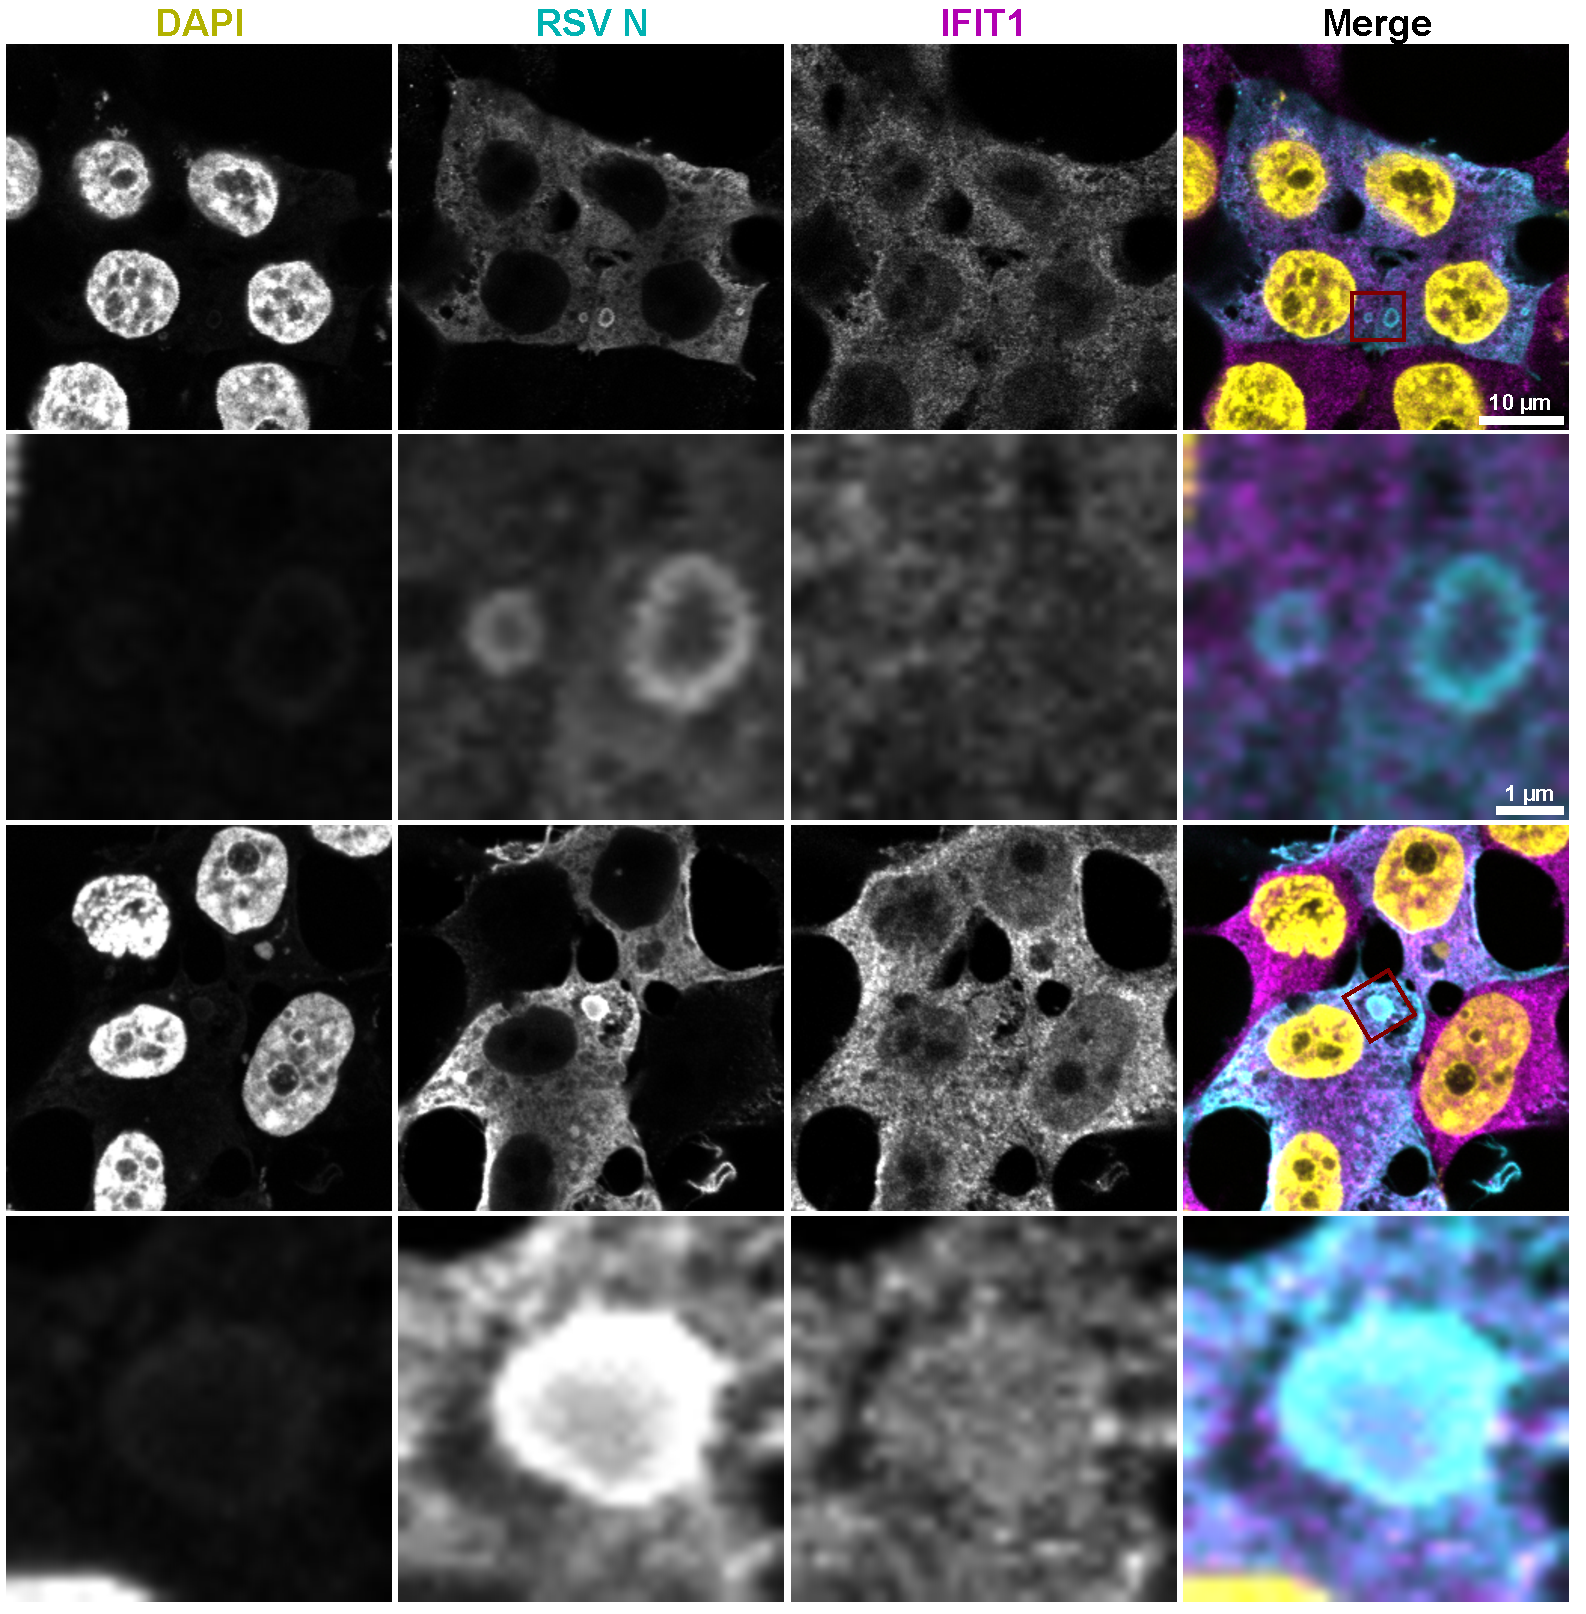
\includegraphics[width=1\linewidth]{09. Chapter 4/Figs/03. IFIT1/01. endo_human.pdf}
    \caption[i1 293t hnhp]{i1 293t hnhp}
    \label{fig:i1 293t hnhp}
\end{figure}

Detecting magenta: endogenous human IFIT1 \newline
Detecting cyan: human pIB \newline
Cell Line: 293T \newline
Treatment: hNhP \newline

Nascent human IFIT1 seems to be diffused through the pIB structure i.e., the signal intensity and distribution between cytoplasmic and pIB staining is identical.  

%vero hnhp
Detecting magenta: endogenous monkey IFIT1 \newline
Detecting cyan: human pIB \newline
Cell Line: VERO \newline
Treatment: hNhP \newline

Endogenous monkey IFIT1 displays colocalization with human pIB structures (top panel), or inclusion within the structures (bottom panel). Monkey IFIT1 signal is also excluded from the pIB filamentous network (top panel; shown by arrows). This suggests that the colocalization is not caused by mere interaction with N or P but its dependant on the integrity of pIBs. These data are supported by z stack measurements.  

\begin{figure}
    \centering
    \includegraphics[width=1\linewidth]{09. Chapter 4/Figs/03. IFIT1/02. endo_monkey.pdf}
    \caption[i1 vero hnhp]{i1 vero hnhp}
    \label{fig:i1 vero hnhp}
\end{figure}


%vero bnbp
Cell Line: VERO \newline
Treatment: bNbP \newline
Detecting magenta: endogenous monkey IFIT1 \newline
Detecting cyan: bovine pIB \newline

In the context of bovine pIB structures, nascent monkey IFIT1 seems to colocalise with the edges of the structures (highlighted by the arrows). Consistent to human pIB data, nascent monkey IFIT1 is excluded from filamentous pIB network.


\begin{figure}
    \centering
    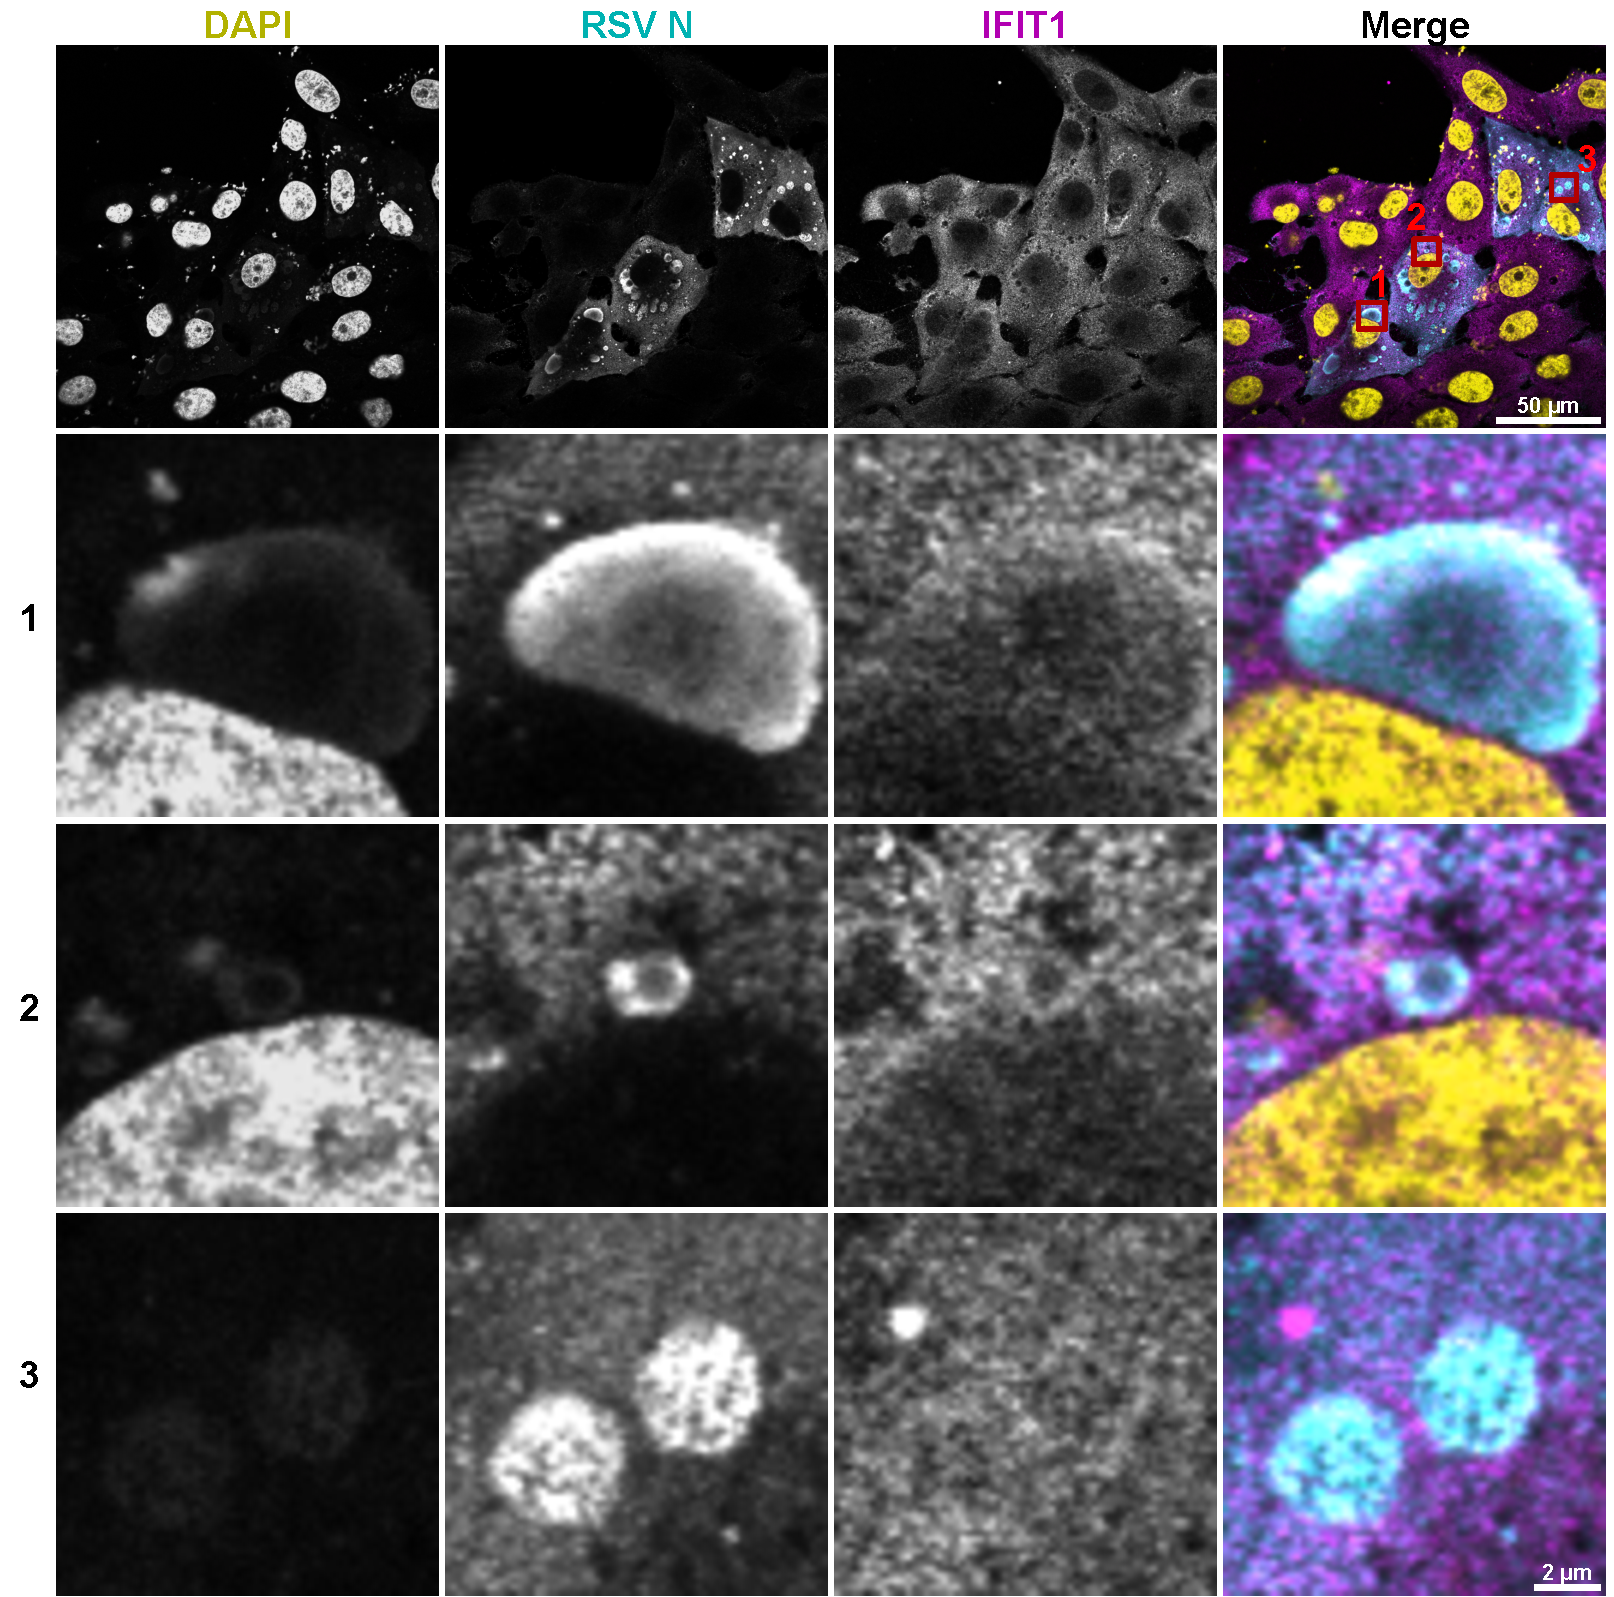
\includegraphics[width=1\linewidth]{09. Chapter 4/Figs/03. IFIT1/03. endo_monkey_bovine-pIB.pdf}
    \caption[i1 vero bnbp]{i1 vero bnbp}
    \label{fig:i1 vero bnbp}
\end{figure}

\subsubsection{Nascent IFIT1 Localisation in the Context of IBs} \label{Nascent IFIT1 Localisation in the Context of IBs}
%hIFIT1 Localisation During hRSV Infection
%a549 hrsv
Detecting magenta: endogenous human IFIT1 \newline
Detecting cyan: human IB \newline
Cell Line: A549 \newline
Treatment: hRSV \newline

Nascent human IFIT1 shows several distinct phenotypes with respect to the hRSV IB interaction. IFIT1 is either concentrated inside the structure (top panel), concentrated on the edge of IB ring (2nd and 3rd panels)  , excluded from the IB structure (4th panel),  or is diffused evenly between the cytoplasm and IB structure (bottom panel).

\begin{figure}
    \centering
    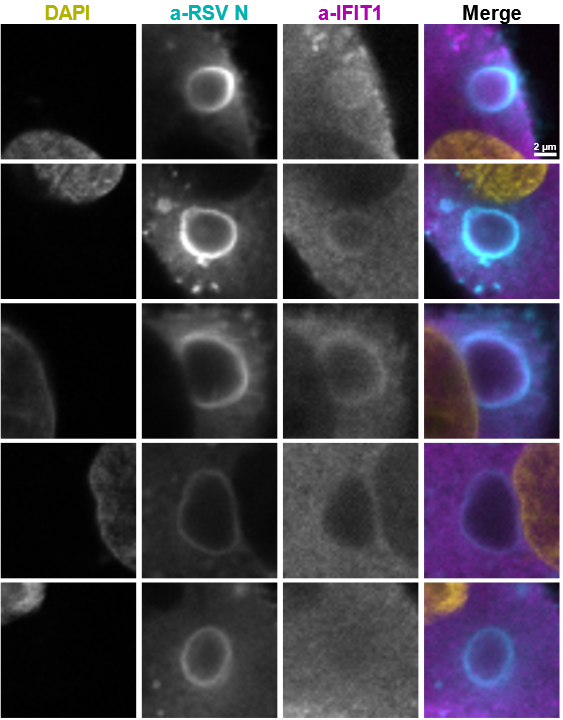
\includegraphics[width=1\linewidth]{09. Chapter 4/Figs/03. IFIT1/04. human infection.png}
    \caption[i1 a549 hrsv]{i1 a549 hrsv}
    \label{fig:i1 a549 hrsv}
\end{figure}


%beas2b hrsv
Detecting magenta: endogenous human IFIT1 \newline
Detecting cyan: human IB \newline
Cell Line: BEAS2B \newline
Treatment: hRSV \newline

\begin{figure}
    \centering
    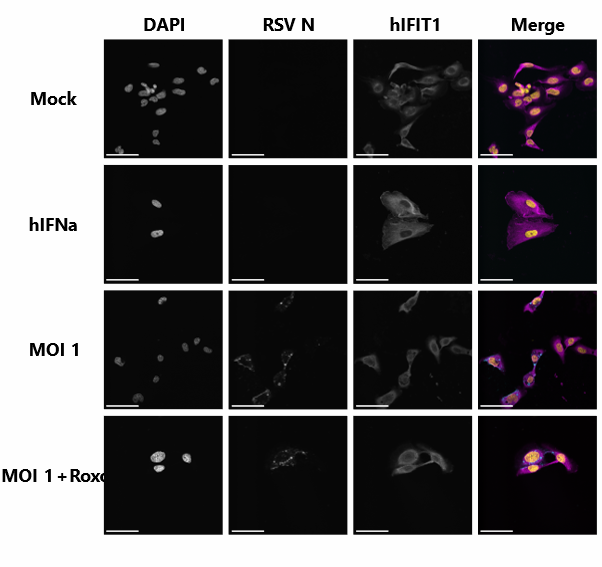
\includegraphics[width=1\linewidth]{09. Chapter 4/Figs/03. IFIT1/05. beas2b hrsv.png}
    \caption[i1 beas2b hrsv]{i1 beas2b hrsv}
    \label{fig:i1 beas2b hrsv}
\end{figure}

%bIFIT1 Localisation During h/bRSV Infection
%mdbk brsv
Detecting magenta: endogenous bovine IFIT1 \newline
Detecting cyan: bovine IB \newline
Cell Line: MDBK \newline
Treatment: bRSV dSH + bIFNa \newline

Nascent bovine IFIT1 in the context of bRSV infection has been observed to localise with the respect of IB in three distinct spaces. We observed it either concentrated inside the central point of the IB structure, while having reduced signal on the inner IB edge, compared to the cytoplasm (top and bottom panels), being excluded from the IB structure (3rd panel), or colocalising on the inner edge of the IB structure while having reduced signal in the middle of the structure compared to cytoplasm, or the edge staining (2nd panel).

\begin{figure}
    \centering
    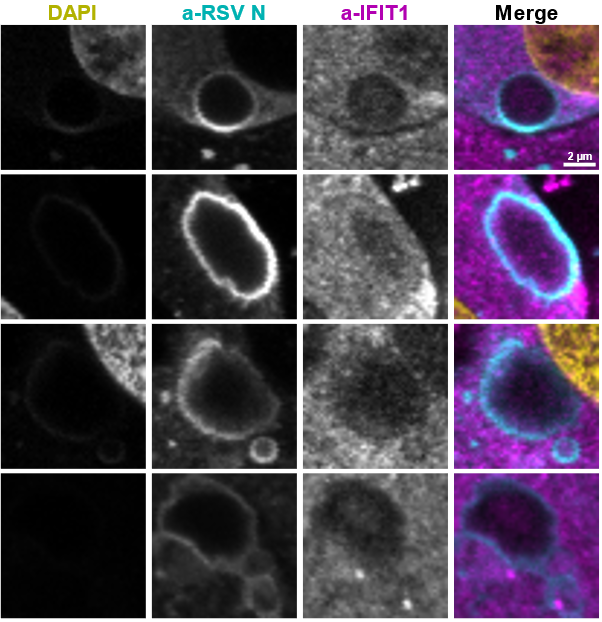
\includegraphics[width=1\linewidth]{09. Chapter 4/Figs/03. IFIT1/06. mdbk brsv.png}
    \caption[i1 mdbk brsv]{i1 mdbk brsv}
    \label{fig:i1 mdbk brsv}
\end{figure}

\subsubsection{Exogenous hIFIT1-FLAG During RSV Infection} \label{Exogenous hIFIT1-FLAG During RSV Infection}
%hi1 + hrsv brsv
Detecting magenta: exogenous human IFIT1-FLAG \newline
Detecting cyan: h/bIB \newline
Cell Line: VERO \newline
Treatment: h/bRSV-GFP \newline

Overexpressed hIFIT1-FLAG colocalises with both human and bovine RSV IBs. This data is supported by evidence from z stacks.

\begin{figure}
    \centering
    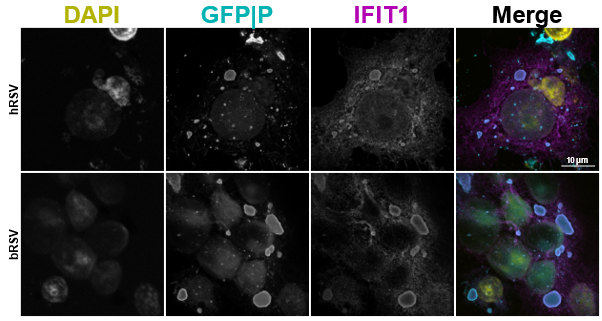
\includegraphics[width=1\linewidth]{09. Chapter 4/Figs/03. IFIT1/07. hi1 hrsv brsv.png}
    \caption[hi1 + hrsv brsv]{hi1 + hrsv brsv}
    \label{fig:hi1 + hrsv brsv}
\end{figure}

\subsubsection{Summary} \label{Summary-i1}
Endogenous human IFIT1 seems to be diffused through the human pIB structure. On the other hand, endogenous monkey IFIT1 forms an inclusion in human pIBs, colocalises with the edge of human and bovine pIBs and is excluded from the filamentous pIB network. This suggests that the colocalization is not caused by mere interaction with N or P but its dependant on the integrity of pIBs. In the context of infection, endogenous human IFIT1 concentrates within the human RSV IB structure; colocalises to the edge of the IB; is diffused through the structure and cytoplasm equally; or is excluded from the structure. This suggests that the interaction between human IFIT1 and hRSV IB is dynamic and depends on factors that we do not understand yet. In the case of endogenous bovine IFIT1 in the context of bRSV IBs, IFIT1 is either excluded from the structure; excluded from the IB inner edge but concentrated inside; or excluded from the centre of IB structure but concentrated on the inner edge of the structure. Overexpressed hIFIT1-FLAG in the context of h/bRSV infection colocalises to both human and bovine IB structures.